\documentclass{report}


\usepackage{minted}
\usepackage{geometry}
\geometry{tmargin=0.5in}
\usepackage{titlesec}
\titleformat{\chapter}[display]
  {\normalfont\bfseries}{}{0pt}{\Large}
\usepackage{Typocaps,lettrine}
\usepackage{graphicx,float}
\graphicspath{ {./} }
\usepackage{subfig}
\usepackage{amsmath, amsthm, amsfonts, amssymb, mathtools}
\usepackage[export]{adjustbox}
\usepackage{enumitem}
\usepackage{chapterbib}
\usepackage[ruled]{algorithm2e}
\usepackage{caption}
\usepackage{float}
\usepackage{makeidx}
\usepackage{hyperref}%
\hypersetup{
	colorlinks = true,
	linkcolor = blue,
}

\title{Documentation of 461 Drawing Project}
\author{Longwood Spring 2021 CS Senior Seminar Students}

\begin{document}
\maketitle
\tableofcontents
\newpage
\section{Preface}
This compilation of documentation exists as a reference for students in the CMSC 461 Senior Seminar course at Longwood University. The Following code has been created by all the students of the class, and an attempt has been made to make a cross platform application that is useful and simple, and document it in a detailed manner.
\chapter{System Dependencies}
  \section{For Linux:}
  \subsubsection*{To get QT:}
    \begin{itemize}
      \item sudo apt get update
      \item sudo apt get upgrade
      \item sudo apt install gt5-default
    \end{itemize}
    \subsection*{To get pdflatex}
    In order to use the LaTeX tool in the app you must have the pdflatex tool downloaded, this can be retrieved from https://miktex.org/download and click over to MacOS and click download

  \bigskip
  \section{For Windows:}
  \subsubsection*{To get QT:}
    \begin{itemize}
      \item Go to www.qt.io
      \item Click “Download. Try.”
      \item Scroll down and click “Go open source”
      \item Scroll down to the bottom and click “Download the Qt Online installer”
      \item Scroll down and click “download”
      \item Open the downloaded program
      \item Follow installers instructions
      \item Make sure to click “Default Qt 5.15 desktop installation”
    \end{itemize}
    \subsection{To get pdflatex}
    In order to use the LaTeX tool in the app you must have the pdflatex tool downloaded, this can be retrieved from https://miktex.org/download and clicking download.

  \bigskip
  \section{For MacOS:}
  \subsubsection*{To get QT:}
    \begin{itemize}
      \item Go to https://www.qt.io click on "Download. Try."
      \item Scroll down and click on "Go open source"
      \item Scroll down and click on "Download the Qt Online Installer"
      \item Click "Download"
    \end{itemize}
    \subsection*{To get pdflatex}
    In order to use the LaTeX tool in the app you must have the pdflatex tool downloaded, this can be retrieved from https://miktex.org/download and click over to MacOS and click download.

\input{jsonProtocol}
\chapter{Client}
  The following is an explanation of the client side of the 461 Drawing Project \linebreak \linebreak

\section{ItemStats}
\subsection{.h}
  itemStats is a struct which contains all of the values which a shape/object
contains. This is used in other documents and functions to help parse out and
separate data.
\begin{minted}
[
frame=lines,
framesep=2mm,
baselinestretch=1.2,
fontsize=\footnotesize,
]
{cpp}
struct itemStats
{
	//Lines get tracked the same as everything else.
	//Set the width/height variables to x2 and y2, respectively.
	std::string board_id;
        std::string type;
        int id;
        double x;
        double y;
        double height;
        double width;
        QColor rgb;

	//Functions to turn the thing into a QJsonObject
	//and a QByteArray that can be sent directly over a socket.

  QJsonObject toJson();
	QByteArray byteData();

	//Several different constructors for a couple of different
	//uses. You can pass in nothing, a QGraphicsItem* for the
	//client end, or a bunch of variables that it will simply
	//insert.
	itemStats();
	itemStats(std::string board_id, QGraphicsItem* item);
	itemStats(std::string board_id, std::string type, int id, double x, double y, \
  double height, double width, QColor rgb);
  ~itemStats();
};
\end{minted}

\subsection{.cpp}
\begin{minted}
[
frame=lines,
framesep=2mm,
baselinestretch=1.2,
fontsize=\footnotesize,
]
{cpp}
itemStats::itemStats(std::string nboard_id, std::string ntype, int nid, double nx, double ny, \
double nheight, double nwidth, QColor nrgb)
  //UPDATE THIS IF YOU ADD THINGS TO THE PLACED ITEMS

itemStats::itemStats(std::string nboard_id, QGraphicsItem* item)
  /*UPDATE THIS IF YOU ADD THINGS TO THE PLACED ITEMS
  Parses the QGraphicsItem and throws the variables into their appropriate places.*/

itemStats::~itemStats()
  //destructor for itemStats

QJsonObject itemStats::toJson()
  /*UPDATE THIS IF YOU ADD THINGS TO THE PLACED ITEMS
  Turns the item into a JSON object, formatted as it would be
  in the jsonExamples folder. This doesn't actually differ at
  all from different shape types.

  For the 'end' parameter, it uses the width and height as x and y coordinates.
  If the thing's a line, the end is just what it says on the tin - the ending coordinates of the line. */

QByteArray itemStats::byteData()
  /*Turns it first into a JSON object, then passes that object
	into a QByteArray. This array can be sent straight to the server.*/

\end{minted}

\section{ProjectScene}
\subsection{.h}
  projectScene is a class which contains functions that relate to the QGraphicsScene,
that is, the 'behinds the scenes' of the graphical window.
\begin{minted}
[
frame=lines,
framesep=2mm,
baselinestretch=1.2,
fontsize=\footnotesize,
]
{cpp}
class ProjectScene : public QGraphicsScene
{
	Q_OBJECT
	private:
		QTcpSocket* m_socket;
		std::vector<itemStats> m_tracked_items;
		std::string m_board_id;

	public slots:
		void sceneChanged(const QList<QRectF> &region);
		void readSocket();
		void disconnect();
	signals:
	public:
                int trackItem(QGraphicsItem* item);
		ProjectScene();
		~ProjectScene();
};

\end{minted}

\subsection{.cpp}
\begin{minted}
[
frame=lines,
framesep=2mm,
baselinestretch=1.2,
fontsize=\footnotesize,
]
{cpp}
  ProjectScene::ProjectScene()
    //A constructor for the ProjectScene class

  ProjectScene::~ProjectScene()
    //A destructor for the ProjectScene class

  ProjectScene::readSocket()
    //Reads in data that is received from the server into a JSON object

  ProjectScene::disconnect()
    /*Deletes the socket from the scene, effectively removing the connection from
      the server.*/

  ProjectScene::trackItem()
    /*Pushes back all the data from a received graphics item into an internal list
      of graphics items.*/

  ProjectScene::sceneChanged()
    /*When something in the scene changes, this event is triggered. What we do is
     get a list of items that have changed (compare between the last update and
     our internal list) and then tells the server about it.*/
\end{minted}

\section{ProjectView}
\subsection{.h}
  projectView is a class which contains the functions which relate to the QGraphicsView,
that is, the canvas and buttons that we see on the graphical window.
\begin{minted}
[
frame=lines,
framesep=2mm,
baselinestretch=1.2,
fontsize=\footnotesize,
]
{cpp}
class ProjectView : public QGraphicsView
{
	Q_OBJECT
	private:
		int m_tool;
		int m_color_r;
		int m_color_g;
		int m_color_b;

        QPointF firstClick;
	private slots:

	public:
		void change_tool(int tool);
		void change_color(int r, int g, int b);

        void circle_tool(qreal x, qreal y,qreal x2, qreal y2);
        void line_tool(qreal x, qreal y, qreal x2, qreal y2);
		void rect_tool(qreal x, qreal y, qreal x2, qreal y2);
		void mousePressEvent(QMouseEvent* event);
		void mouseReleaseEvent(QMouseEvent* event);
		ProjectView();
		~ProjectView();
};
\end{minted}


\subsection{.cpp}

\begin{minted}
[
frame=lines,
framesep=2mm,
baselinestretch=1.2,
fontsize=\footnotesize,
]
{cpp}
ProjectView::ProjectView()
  //A constructor for the ProjectView class

ProjectView::~ProjectView()
  //A destructor for the ProjectView class

ProjectView::change_tool(int tool)
  //Change the current tool based on an integer parameter

ProjectView::change_color(int r, int g, int b)
    //Change the current tool's color based on 3 integer parameters, r, g, and b.

ProjectView::circle_tool(qreal x, qreal y, qreal x2, qreal y2)
  /*Draw a circle on the canvas using two points, (x,y) and (x2,y2). This allows
    us to draw ellipses easily as well as circeles, similarly to how we draw
    rectangles.
    (x,y) is the first location the user clicked, and (x2,y2) is the second.*/

ProjectView::line_tool(qreal x, qreal y, qreal x2, qreal y2)
    /*Draw a line on the canvas using two points, (x,y) and (x2,y2).
    (x,y) is the first location the user clicked, and (x2,y2) is the second.*/

ProjectView::rect_tool(qreal x, qreal y, qreal x2, qreal y2)
    /*Draw a rectangle on the canvas using two points, (x,y) and (x2,y2).
    (x,y) is the first location the user clicked, and (x2,y2) is the second.*/

ProjectView::mousePressEvent()
     /*This event is triggered when the user clicks down on the mouse. Technically,
     it stores this point and doesn't do anything with it until a mouseReleaseEvent.*/

ProjectView::mouseReleaseEvent()
    /*This event is triggered when the user releases the click on the mouse. This
    function takes the second point, figures out which action to take based on
    the selected tool, and calls the appropriate function.*/
\end{minted}

\section{ToolBar}
\subsection{.h}
  toolbar is a class which contains the functions to change the different tools in
the graphical window.
\begin{minted}
[
frame=lines,
framesep=2mm,
baselinestretch=1.2,
fontsize=\footnotesize,
]
{cpp}
class ToolBar : public QWidget
{
	Q_OBJECT
	private:
		QPushButton* m_circle;
		QPushButton* m_line;
		QPushButton* m_rect;
		QPushButton* m_default;
		QPushButton* m_black;
		QPushButton* m_red;
		QPushButton* m_green;
		QPushButton* m_yellow;
		QPushButton* m_blue;
		QPushButton* m_color_picker;
		QVBoxLayout* m_layout;
		ProjectView* m_view;
	public slots:
		// set default
        	void set_default();
        	// shapes
        	void place_rectangle();
        	void set_line();
        	void set_circle();
        	// colors
        	void set_color_black();
        	void set_color_red();
        	void set_color_green();
        	void set_color_yellow();
        	void set_color_blue();
        	void set_color_custom();

	public:
		ToolBar();
		~ToolBar();
		void set_view(ProjectView* view);

};
\end{minted}

\subsection{.cpp}
\begin{minted}
[
frame=lines,
framesep=2mm,
baselinestretch=1.2,
fontsize=\footnotesize,
]
{cpp}
ToolBar::ToolBar()
  //A constructor for the ToolBar class

ToolBar::~ToolBar()
  //A destructor for the ToolBar class

ToolBar::set_view(ProjectView* view)
  //Sets the tool's m_view to view

ToolBar::set_default()
  //Sets the default tool to the select tool

ToolBar::set_line()
  //Sets the tool to the line tool

ToolBar::set_circle()
  //Sets the tool to the circle tool

ToolBar::set_rect()
  //Sets the tool to the rect tool

ToolBar::set_color_black()
  //Sets the tool's color to be black

ToolBar::set_color_red()
  //Sets the tool's color to be red

ToolBar::set_color_green()
  //Sets the tool's color to be green

ToolBar::set_color_yellow()
  //Sets the tool's color to be yellow

ToolBar::set_color_blue()
  //Sets the tool's color to be blue



ToolBar::set_color_custom()
  /*Brings up a color picker menu for the user to set their own color using a
    graphical interface, rgb, hexadeicimal, or cmyk.*/
\end{minted}

\section{Window}
\subsection{.h}
  window is essentially the 'main' of the graphical window, though there is a
'main' that spawns it.
\begin{minted}
[
frame=lines,
framesep=2mm,
baselinestretch=1.2,
fontsize=\footnotesize,
]
{cpp}
class Window : public QMainWindow //Extension on the base QMainWindow class
{
	Q_OBJECT //Must be included for qmake to recognize this

	private: //Menus and features of the window
		ToolBar* m_bar;
		QDockWidget* m_tool_dock;
		ProjectScene* m_scene;
		ProjectView* m_view;

        // shape tools

	private slots: //Where functions attached to buttons go
        // make a popup window
		void popup();
	public:
		Window();
		~Window();
};
\end{minted}

\subsection{.cpp}
\begin{minted}
[
frame=lines,
framesep=2mm,
baselinestretch=1.2,
fontsize=\footnotesize,
]
{cpp}
Window::Window()
  /*A constructor for the Window class. Sets up the entire graphical window with
    toolbars, docks, a canvas, a scene, and a menu.*/

Window::~Window()
  //A destructor for the Window class.
\end{minted}

\section{Main}
\subsection{.cpp}
  main.cpp is a small file which contains one function: int main. This is the start of
the entire client, where a new window is created in memory and executed. From
there, upon returning, the event loop begins.
\begin{minted}
[
frame=lines,
framesep=2mm,
baselinestretch=1.2,
fontsize=\footnotesize,
]
{cpp}
int main(int argc, char* argv[])
  /*This is the start of the entire client, where a new window is created in memory and executed.*/
\end{minted}

\chapter{Server}
  The server is run off of a Qt framework using Qt sockets. Clients can connect to the server via these Qt sockets, and are assigned unique identifiers using the socketDescriptor value of the connecting socket. By maintaining a constant connection, the server is able to receive and send the most current information about databases and shapes.

\section*{Server}
\addcontentsline{toc}{section}{\protect\numberline{}Server}%
\subsection{.h}
Server.h includes some tools to set up an item based on its data and turn it into a byte array. Also turn it into a QJsonObject.
\begin{minted}
[
frame=lines,
framesep=2mm,
baselinestretch=1.2,
fontsize=\footnotesize,
]
{cpp}
struct ownedDB{
    int id;
    QSqlDatabase db;
} newDB;

class Server : public QMainWindow
{
	Q_OBJECT
	private:
		QTcpServer* m_server;
		QSet<QTcpSocket*> connected;
		std::string m_board_id;
        QVector<ownedDB> databases;

	public slots:
		void newConnection();
		void readSocket();
		void disconnect();
	public:
		Server();
		~Server();
		void appendSocket(QTcpSocket* sock);
        void createBoard(QTcpSocket* socket);
        void deleteDB(QTcpSocket* socket);
};
\end{minted}

\subsection{.cpp}
\begin{minted}
[
frame=lines,
framesep=2mm,
baselinestretch=1.2,
fontsize=\footnotesize,
]
{cpp}
Server::Server() : QMainWindow()
  /*Sets up the server itself.
  The server will give out a 'signal' when it receives a new connection.
  This connects that signal to the function 'newConnection()'.*/

void Server::newConnection()
  /*Checks for pending connections, then calls the other function that actually adds the socket
	to the list of sockets we have.*/

void Server::appendSocket(QTcpSocket* socket)
  //adds a new socket to all current clients are stored in the vector.

void Server::disconnect()
  //Black voodoo magic with a cast to determine which socket it was that needs to be disconnected.

void Server::readSocket()
  /*There is a QByteArray array of bytes that the socket has just sent to the server.
  The array is formatted as a JSON object. The client sends out this JSON object in
  the exact format that is specified in the jsonExamples folder. The data gets received and is
  ready to be parsed and turned into a string and outputs it to console. Casts the byte array
  into a Qt style JSON object. You can get keys and values out of this the same way
	you would anything else. Qt documentation will have more specific info on:*/

  QJsonDocument doc = QJsonDocument::fromJson(buf);
	QJsonObject obj = doc.object();

void Server::createBoard(QTcpSocket* socket)
      /*Create a QSqlDatabase, either connect to the database named CMSC461.db or
      create it if it doesn't exist. Create and QSqlQuery pointer to be used to execute commands*/

void Server::deleteDB(QTcpSocket* socket)

\end{minted}

\subsection{.py}
\begin{minted}
[
frame=lines,
framesep=2mm,
baselinestretch=1.2,
fontsize=\footnotesize,
]
{python}
  def getJsonFile():

  def addCircle(bid,sid,r,x,y,color):
    #Creates JSON-formatted circle data

  def addLine(bid,sid,x1,y1,x2,y2,color):
    #Creates JSON-formatted line data

  def addRect (bid,sid,x,y,w,h,color):
    #Creates JSON-formatted rectangle data

  @app.route('/addShape', methods = ['POST', 'GET'])
  def shapeType():
    #Checks shape type received and calls matching function

  @app.route('/saveFile', methods = ['POST', 'GET'])
  def saveFile():
    # A implementation of saveFile which allows the user to save the board that they are currently using.
    # User will send this url to the server and server will reply back with an SVG file

  @app.route('/fullUpdate', methods = ['POST', 'GET'])
  def fullUpdate():
    """This function keeps track of all shapes across all clients concurrently via a QByteArray of JSON objects. In order to acquire the information from the SQL database, the function calls queries on the Ellipse, Line, and Rect tables of the database "databaseName" that is passed in by the function call. It then converts them to JSON objects by using the itemStats constructor and then using the .toJson() method. Each JSON object is then placed into the QByteArray. This byte array is then sent to the socket that requested the fullUpdate."""

  @app.route('/createBoard', methods = ['POST', 'GET'])
  def createBoard():
    # Create a new database for every new board that is created
\end{minted}

\section*{Main}
\addcontentsline{toc}{section}{\protect\numberline{}Main}%
\subsection{.cpp}
\begin{minted}
[
frame=lines,
framesep=2mm,
baselinestretch=1.2,
fontsize=\footnotesize,
]
{cpp}
int main(int argc, char* argv[])
\end{minted}

\chapter{User Manual}
This chapter provides an explanation of the canvas and how to manipulate the tools provided. Below is what a blank canvas will look like:
\begin{figure}[h!]
\centering
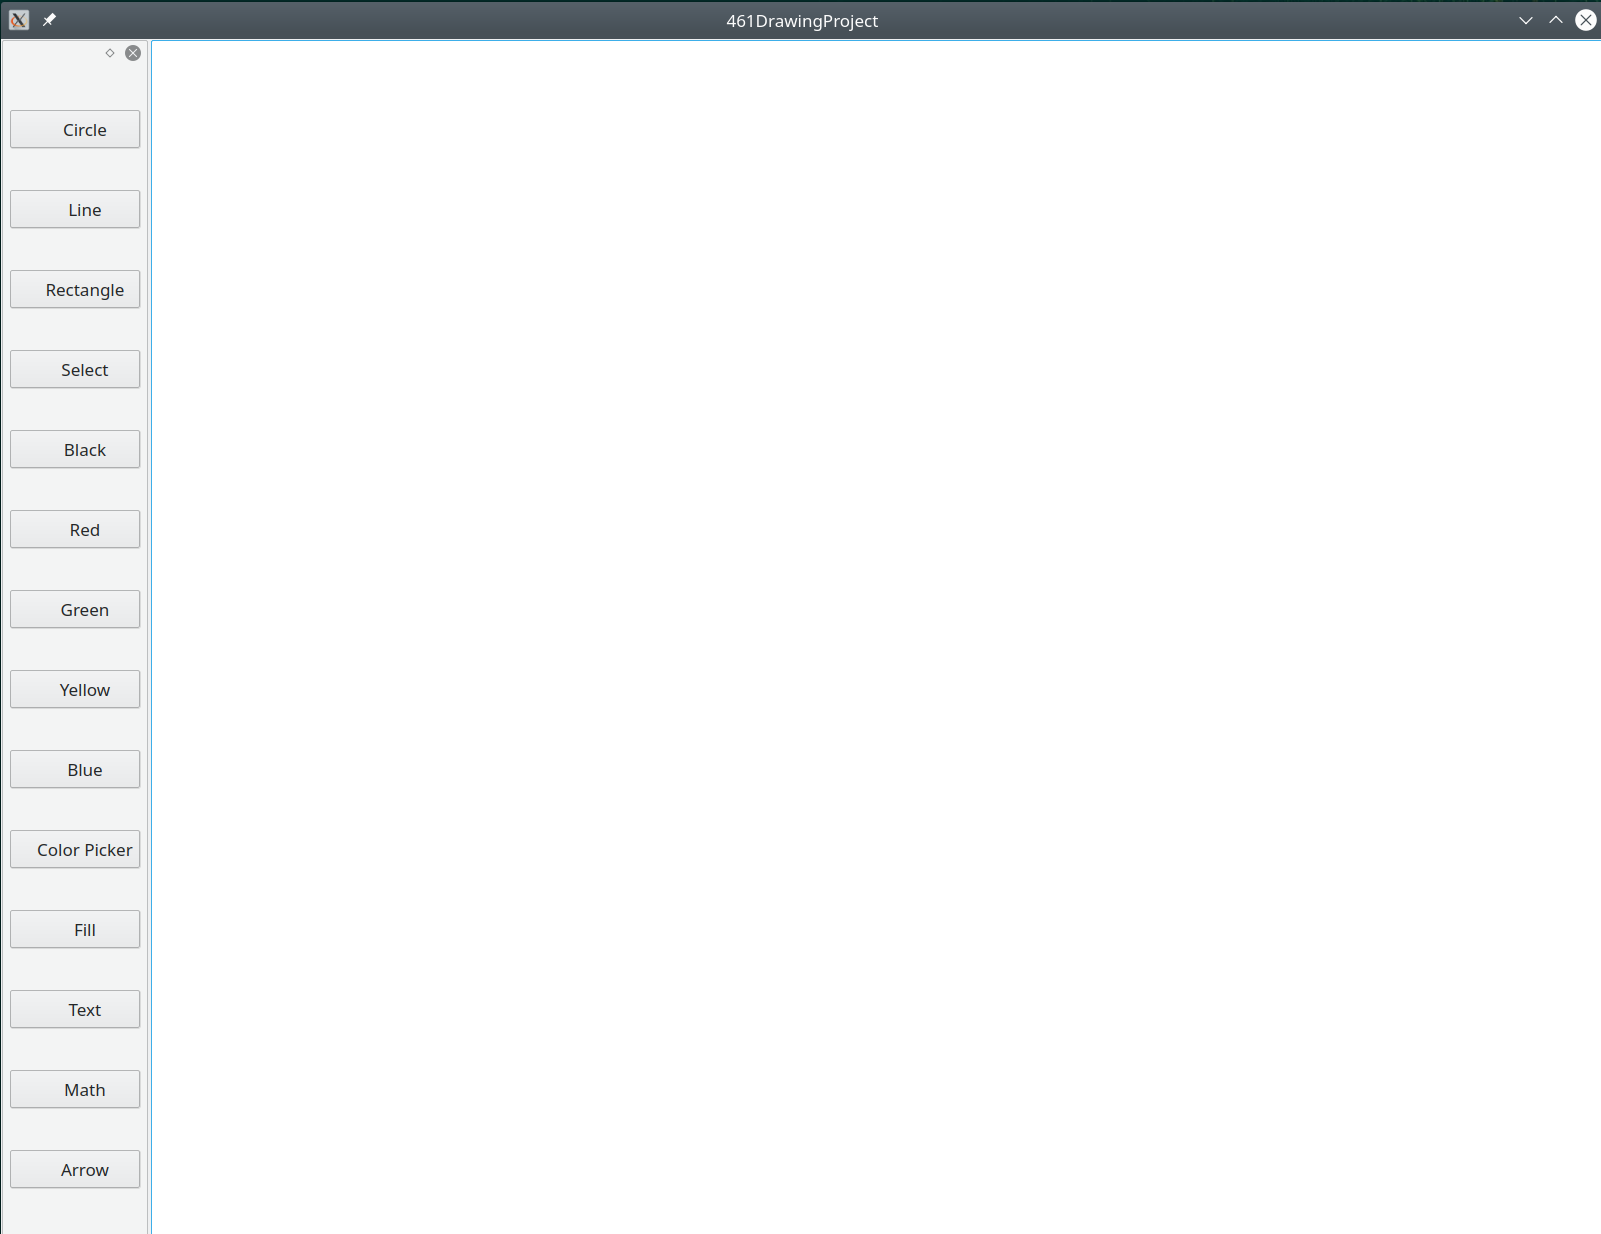
\includegraphics[height=10cm, width=10cm]{canvas}
\caption{Blank Canvas}
\end{figure}

\section{Manipulating Items}
\subsection{Select}
\begin{figure}[h!]

\includegraphics{select}
\end{figure}
  The way to manipulate items drawn on the canvas is to use the "select" tool. With the select tool equipped click, hold, and drag an item to the desired location, then release the item and it will be relocated to its new position.


\section{Drawing}
Below is an explanation on how to use each drawing tool

\subsection{Lines}
\begin{figure}[h!]

\includegraphics{line}
\end{figure}
Select the line button, then on the canvas, click two separate points you want to draw a line between.

\subsection{Rectangles}
\begin{figure}[h!]

\includegraphics{rect}
\end{figure}
Select the rectangle button, then on the canvas, click one point to be the top right corner and click the second point to be the bottom left corner and a rectangle will be drawn in between.

\subsection{Circle}
\begin{figure}[h!]

\includegraphics{circle}
\end{figure}
Select the Circle button, then on the canvas, click two separate points, the first is the center point and the second is the radius. A circle will be drawn using those two reference points.

\subsection{Arrow}
\begin{figure}[h!]

\includegraphics{arrow}
\end{figure}
here will be arrow details

\subsection{LaTeX}
\begin{figure}[h!]

\includegraphics{math}
\end{figure}
Select the Math button, then in the text box type in your desired LaTeX code and click the enter button.

\subsection{Text}
\begin{figure}[h!]

\includegraphics{text}
\end{figure}
Select the text button, then in the text box type in your desired sentence and click the enter button.

\subsection{Changing Colors}
\begin{figure}[h!]

\includegraphics{cp}
\end{figure}
There are two ways to change color of the shapes, the first is to select one the colors on the side bar, the second is to click 'Color Picker' and choose a color based on RGB value.

\subsection{Fill}
\begin{figure}[h!]

\includegraphics{fill}
\end{figure}
  The fill tool is used to fill a shape with a desired color. To use the tool first click the "fill" button then click the desired fill color, and finally click within the boundaries of the shape you want to fill.



\end{document}
